\documentclass[10pt,compress,mathserif]{beamer}
\usetheme{Berkeley}
% Few theme names Berkeley Copenhagen Dresden


\usepackage{amsmath,minibox,amssymb,amsfonts,amsthm,graphicx,color,multirow,array,tikz,hyperref}
\usetikzlibrary{arrows,snakes,backgrounds,patterns,matrix,shapes,fit,calc,shadows, positioning}

\setbeamertemplate{navigation symbols}{} % This is just to get rid of the extra fazool symbols
\setbeamertemplate{caption}{\raggedright\insertcaption\par}

\setbeamerfont{caption}{size=\footnotesize}

\title[]{Control Systems Project}
\author[]{Ali Asghar\\ 21PWCSE2059 \\ Section C DCSE \\ UET Peshawar.}
\rightskip=0pt plus 0pt
\boldmath

\begin{document}

\begin{frame}    \titlepage \end{frame}



% First slide
\section{Introduction}
\begin{frame}{Introduction to Project}
\noindent Perform the following for Problem 22 at Page 148:\\ \vskip10pt
%a. Obtain state-space representation for the system (without obtaining any transfer function). \\ \vskip10pt
%b. Choose the output matrix as you like (except identity matrix - and make the system observable). \\ \vskip10pt
%c. Check the stability of the system using all methods that you know.\\ \vskip10pt
%d. Compute the controllability and observability for the system. If the system is controllable, place the controller poles at (-3, -5) and observer poles at a location which is faster than the controller poles.\\ \vskip10pt
%e. Simulate the system using observer based feedback controller and show all the responses.

a. Consider the state-space of Problem 22, Page 148 of Norman Nise Book Edition 5. \\
b. Check the stability of the system using all the methods that you know. \\
c. Compute the controllability and observability for the system. If the system is unstable, design a suitable controller for it. \\
d. Simulate the system using the controller that you design and show all the responses.\\
e. Design a PID Controller and show the response of the system using PID Controller. Compare the results obtained in part d and e.\\
f. Compute the steady state errors before and after designing controller.\\

\end{frame}

\begin{frame}{Introduction to Project}
	\begin{figure}[h!]
		\centering
		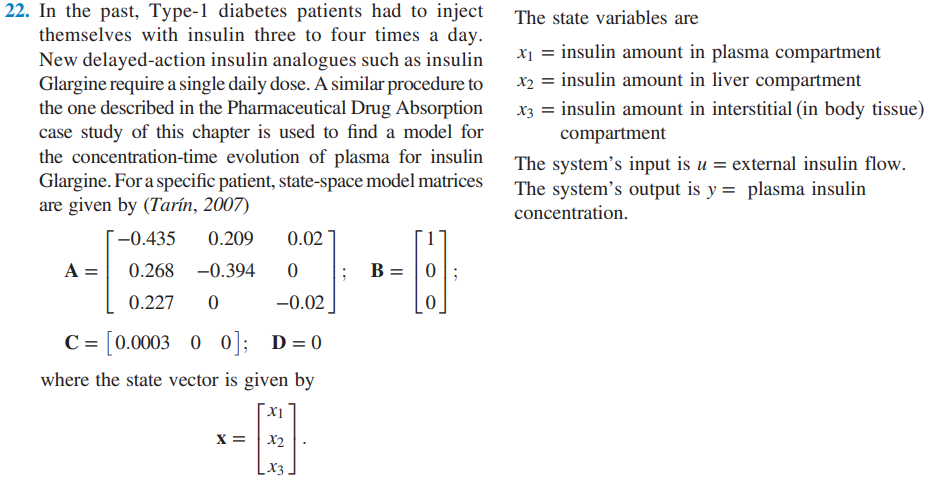
\includegraphics[scale=0.6]{images/Problem22.png}
		\caption{}
	\end{figure}
\end{frame}

% Second Slide
\section{Solution}
\begin{frame}{State-space Representation of the System}
The state-space representation of the system can be written as follows:\begin{equation}
\begin{bmatrix} \dot{x_1}\\  \dot{x_2}\\ \dot{x_3} \end{bmatrix}
= \begin{bmatrix}
-0.435 & 0.209 & 0.02\\
0.268 & -0.394 & 0\\
0.227 & 0 & -0.02\end{bmatrix}
\begin{bmatrix} x_1\\  x_2 \\ x_3 \end{bmatrix} +
\begin{bmatrix}
1 \\
0 \\
0 \end{bmatrix}
u(t)
%\begin{bmatrix} u_1 \end{bmatrix}
\end{equation}

\begin{equation}
y=\begin{bmatrix}
0.003 & 0 & 0
\end{bmatrix}x
\end{equation}

\end{frame}


\section{Stability Analysis}
\begin{frame}{Stability Analysis of the System}

	\begin{figure}[h!]
		\centering
		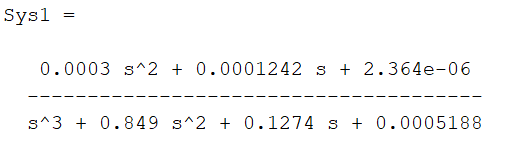
\includegraphics[scale=0.65]{images/tf.png}
		\caption{Transfer Function}
	\end{figure}
	
The eigen values of the system are:
\begin{equation} \lambda_1 = -0.6560,  \lambda_2 = -0.1889, \lambda_3 = -0.0042 \end{equation}
   

The poles of the system are:
\begin{equation} p_1 = -0.6560,  p_2 = -0.1889, p_3 = -0.0042 \end{equation} \vskip10pt

\end{frame}

%\begin{frame}{Stability Analysis of the System}
%Routh-Hurwitz table is shown below
%\begin{table}[h] \begin{center}
%\begin{tabular}{|l|c|l|} \hline
%$s^3$  & 1 & 31 \\ \hline
%$s^2$  & 10 & 31 \\ \hline
%$s^1$  & $-\frac{1}{10}\times\begin{vmatrix} 1 & 31\\ 10 & 31 \end{vmatrix}=27.9$ & 0 \\
%$s^0$  & $-\frac{1}{27.9}\times\begin{vmatrix} 10 & 31\\ 27.9 & 0.1 \end{vmatrix}=31$ & 0 \\ \hline
%\end{tabular} \end{center}
%\end{table}
%As there are no sign changes in the first column, the system is stable.
%\end{frame}


\begin{frame}{Stability Analysis of the System}
	The step response of the system is:
	\begin{figure}[h!]
		\centering
		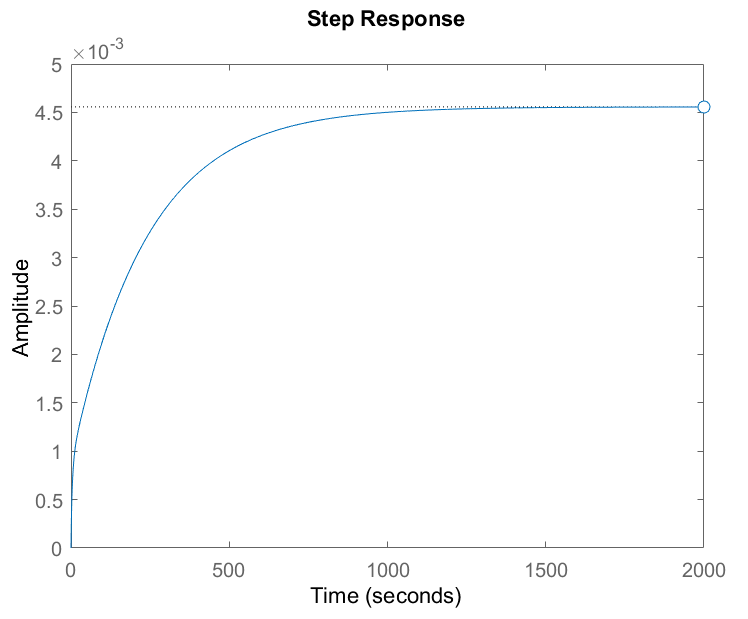
\includegraphics[scale=0.65]{images/stepResponse.png}
		\caption{Plot of step response.}
	\end{figure}
\end{frame}

\begin{frame}{Stability Analysis of the System}
	The Pole-Zero Map of the system is:
	\begin{figure}[h!]
		\centering
		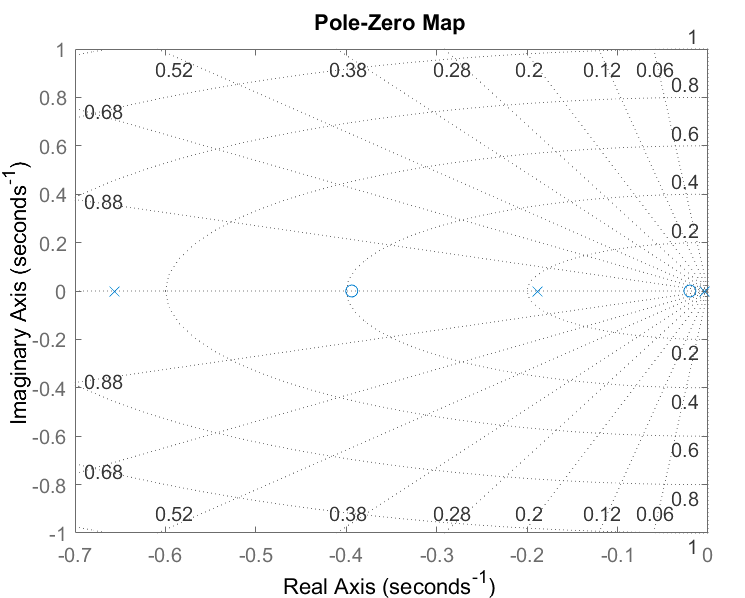
\includegraphics[scale=0.65]{images/poleZeroMap.png}
		\caption{Plot of step response.}
	\end{figure}
\end{frame}

\begin{frame}{Stability Analysis of the System}
	The Root Locus of the system is:
	\begin{figure}[h!]
		\centering
		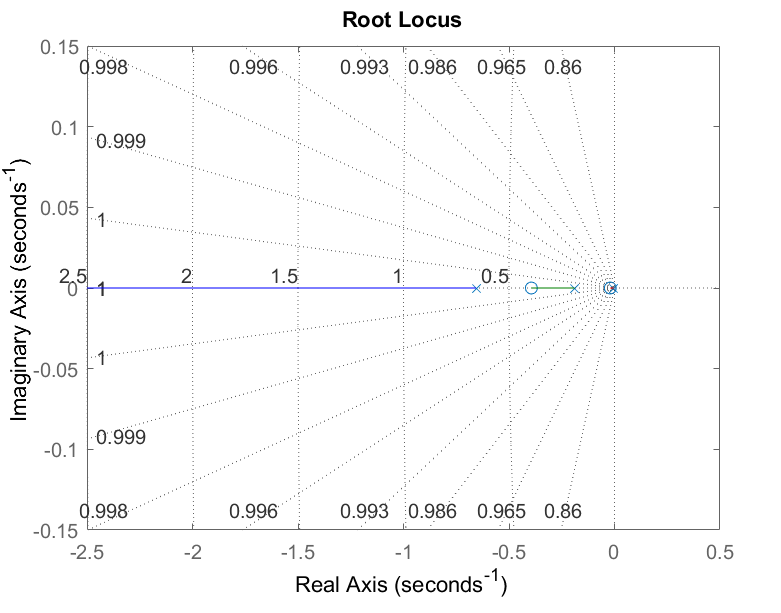
\includegraphics[scale=0.65]{images/rootLocus.png}
		\caption{Plot of step response.}
	\end{figure}
\end{frame}



\section{Controllability and Observability}
\begin{frame}{Controllability and Observability Analysis}
No Need for Controllability and Observability Analysis as the system is stable already.
\end{frame}


%\section{Observability}
%\begin{frame}{Observability Analysis}
%\end{frame}


\section{Controller Design}
\begin{frame}{Controller Design}
	\begin{figure}[h!]
		\centering
		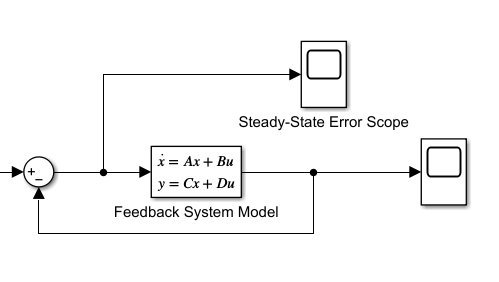
\includegraphics[scale=0.75]{images/SSE_Sketch.png}
		\caption{Steady State Error Computation}
	\end{figure}
\end{frame}

\section{Controller Design}
\begin{frame}{Controller Design}
		
	\begin{figure}[h!]
		\centering
		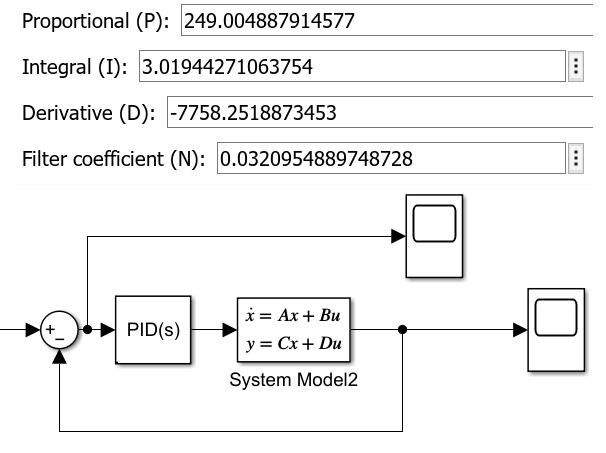
\includegraphics[scale=0.65]{images/PIDController.png}
		\caption{PID Controller Design}
	\end{figure}

\end{frame}


\section{Results}
\begin{frame}{Simulink Results}
Steady-State Error before PID \( \approx 0.9955 \)

\begin{figure}[h!]
	\centering
	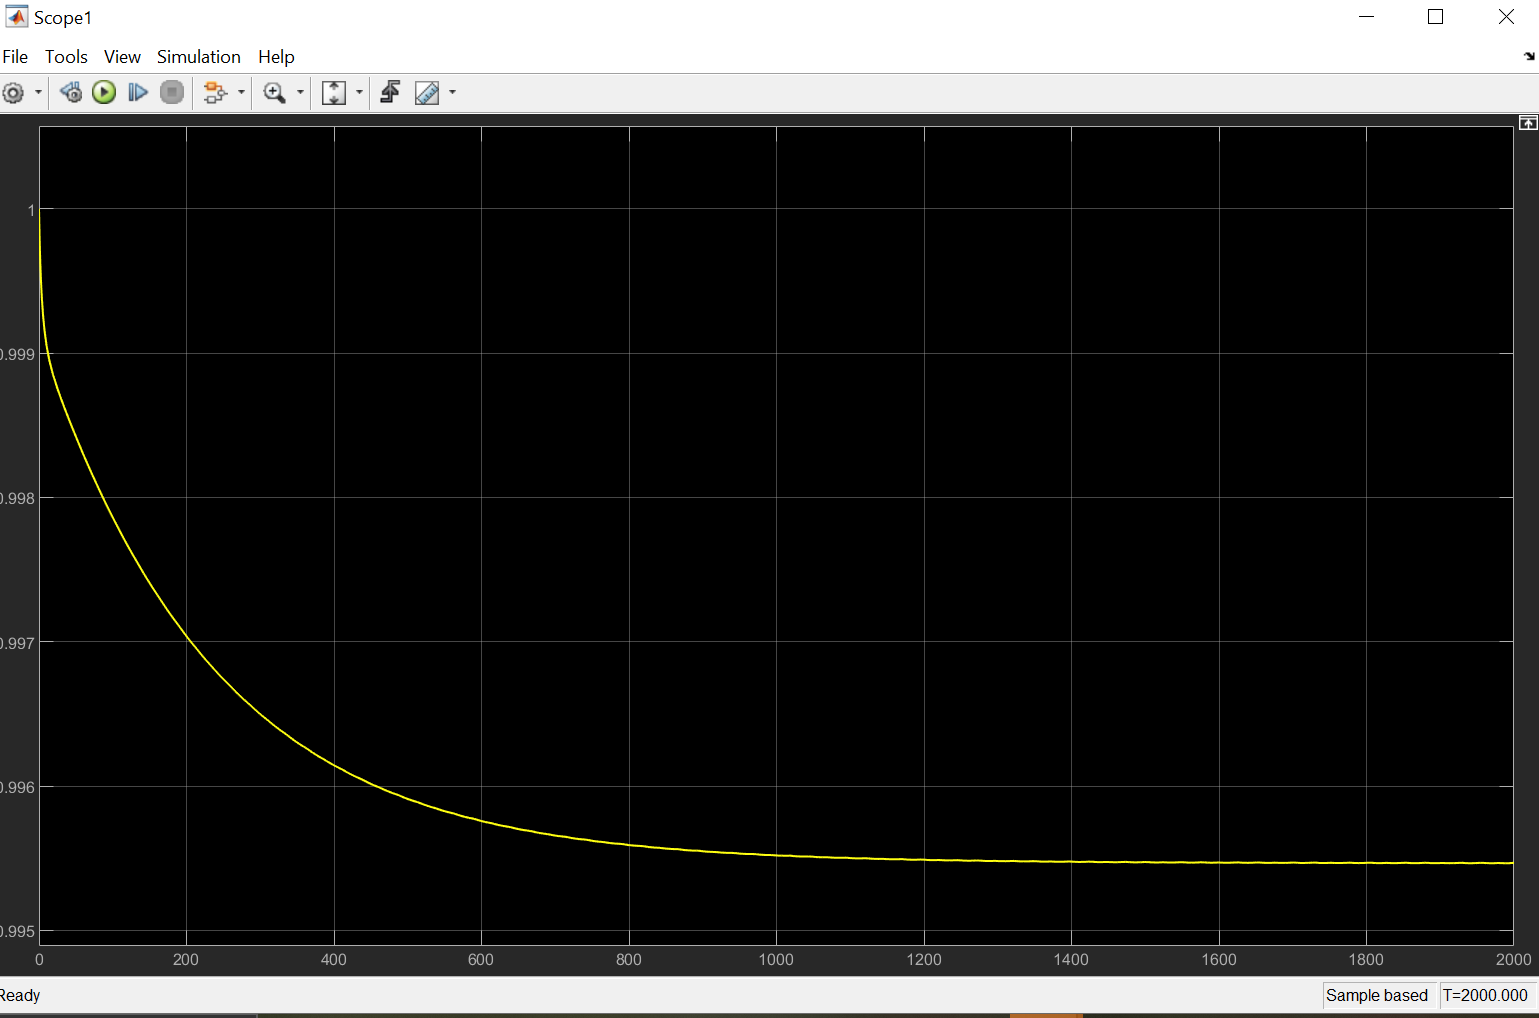
\includegraphics[scale=0.35]{images/SSE_BeforePID_Simulink.png}
	\caption{Plot of SSE Before PID.}
\end{figure}


%Put results without controller and with controller \\ \vskip10pt
%Compute steady state errors and show those errors before controller design, after controller design, and after tracking %controller design \\ \vskip10pt
%Verify the steady state errors from Matlab or Simulink by step response and ramp response (be careful with the magnitude of step input and ramp input - it should be the same as your project question).

\end{frame}

\begin{frame}{Simulink Results}
Steady-State Error After PID \( \approx 0 \)
	\begin{figure}[h!]
		\centering
		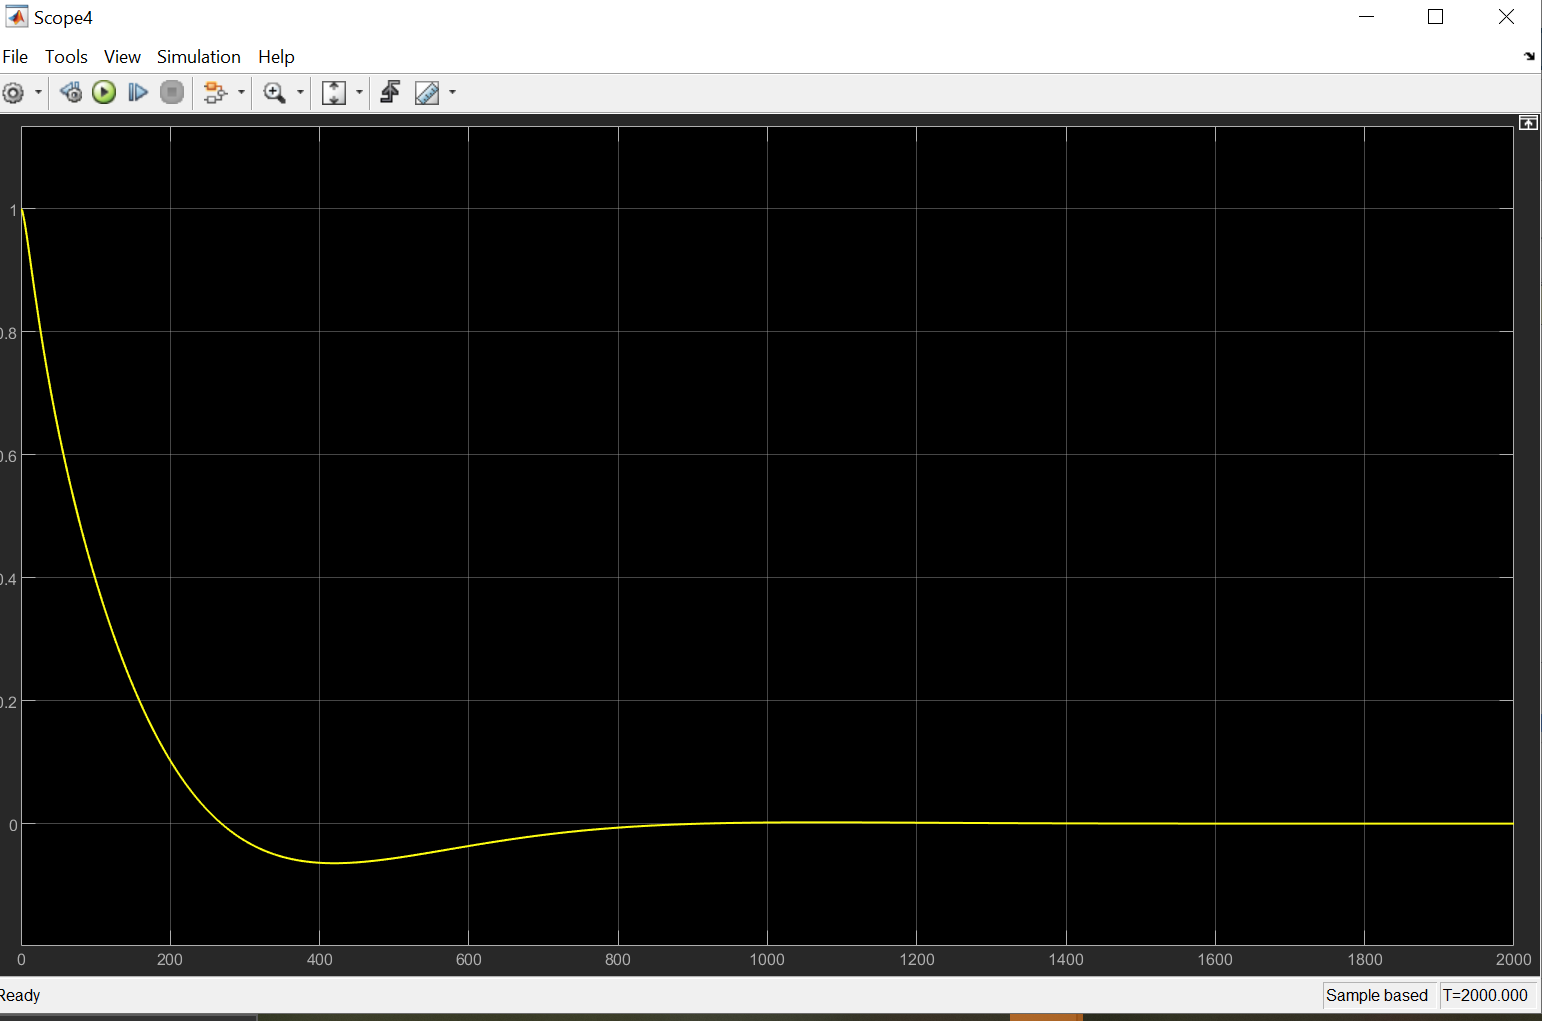
\includegraphics[scale=0.35]{images/SSE_AfterPID_Simulink.png}
		\caption{Plot of SSE after PID}
	\end{figure}
\end{frame}


\begin{frame}{Simulink Results}

	\begin{figure}[h!]
		\centering
		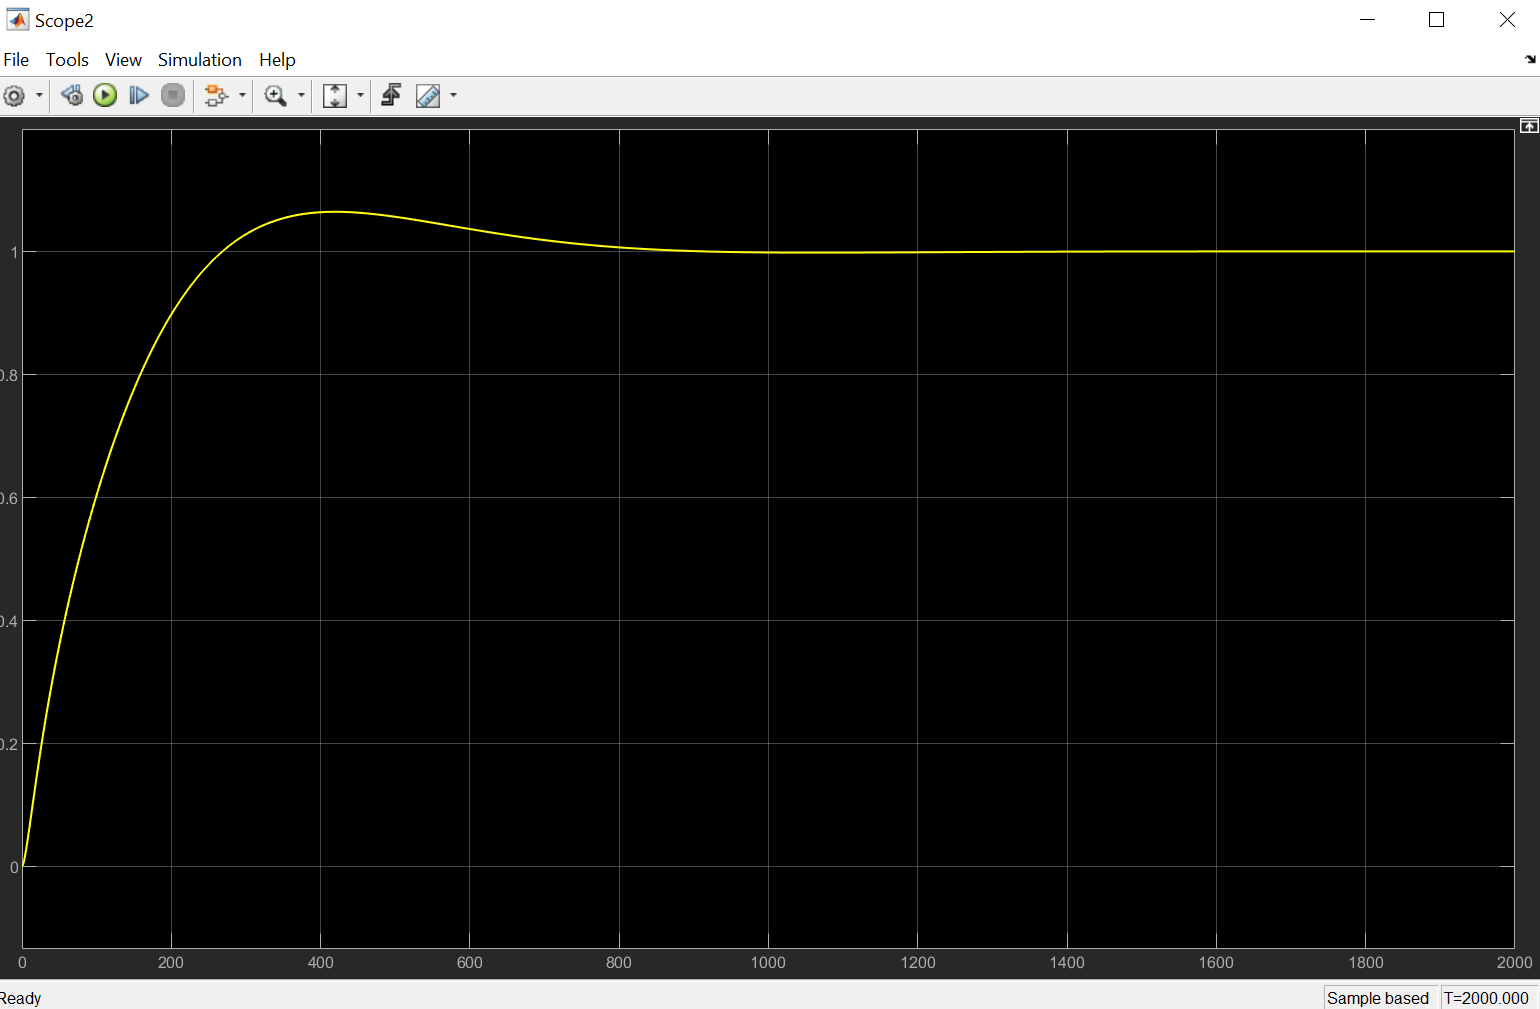
\includegraphics[scale=0.35]{images/stepResponse_PID_Simulink.png}
		\caption{Plot of Step Response in Simulink}
	\end{figure}
\end{frame}

\begin{frame}{Simulink Results}

	\begin{figure}[h!]
		\centering
		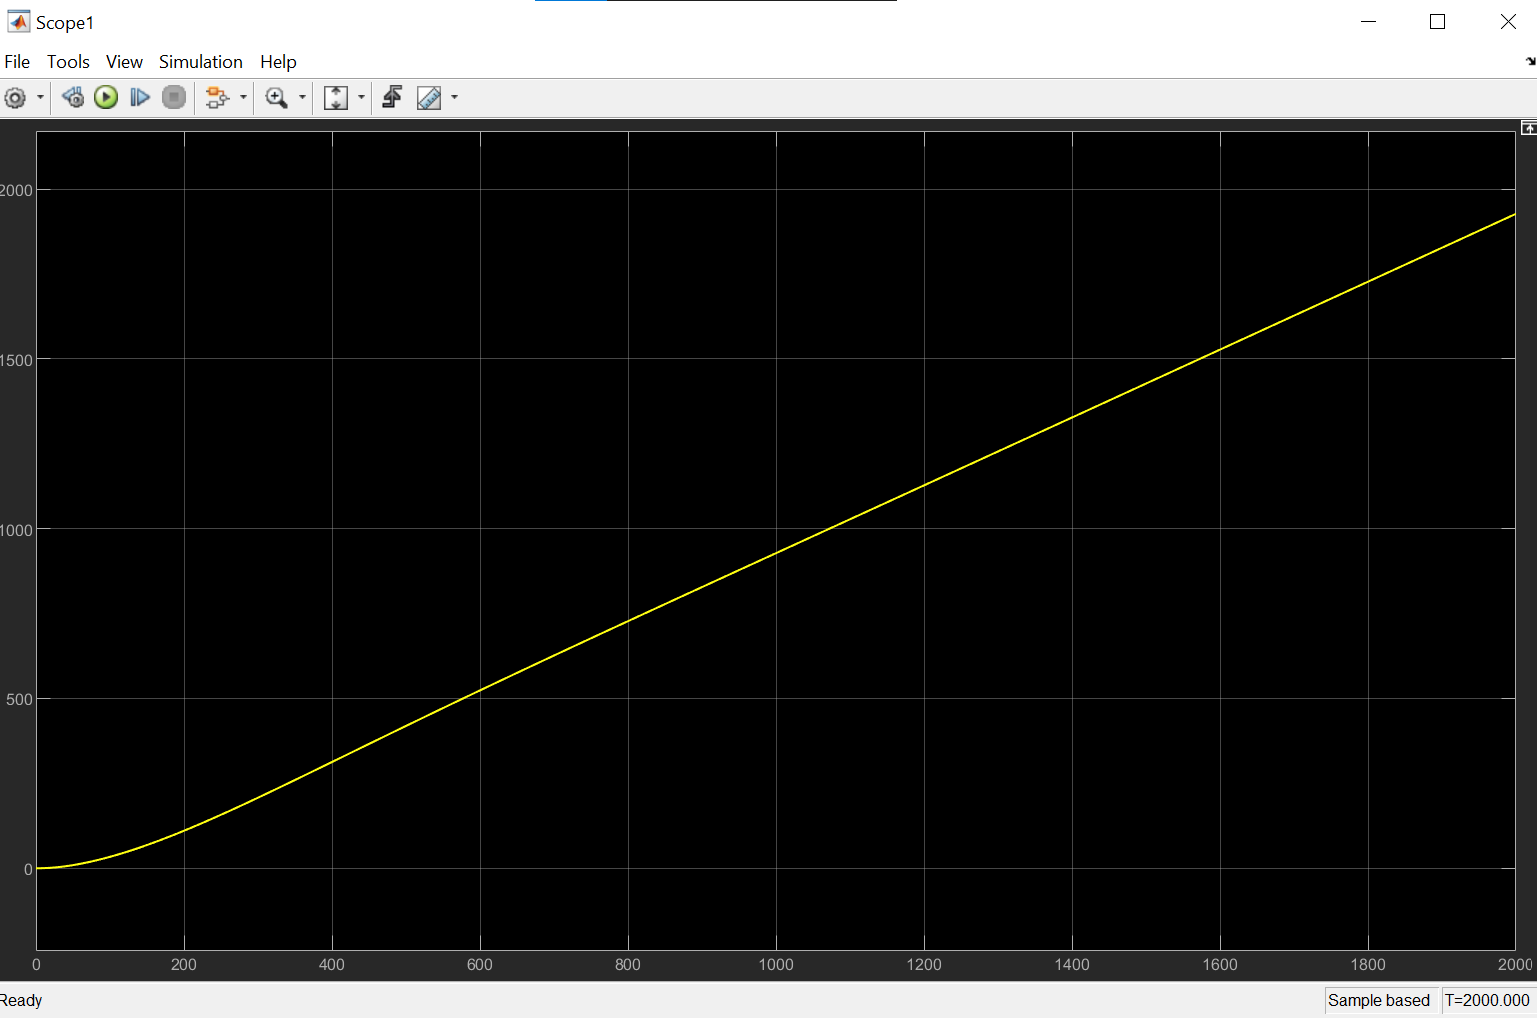
\includegraphics[scale=0.35]{images/rampResponse_PID_Simulink.png}
		\caption{Plot of Ramp Response in Simulink After PID}
	\end{figure}
\end{frame}

\begin{frame}{Simulink Results}

	\begin{figure}[h!]
		\centering
		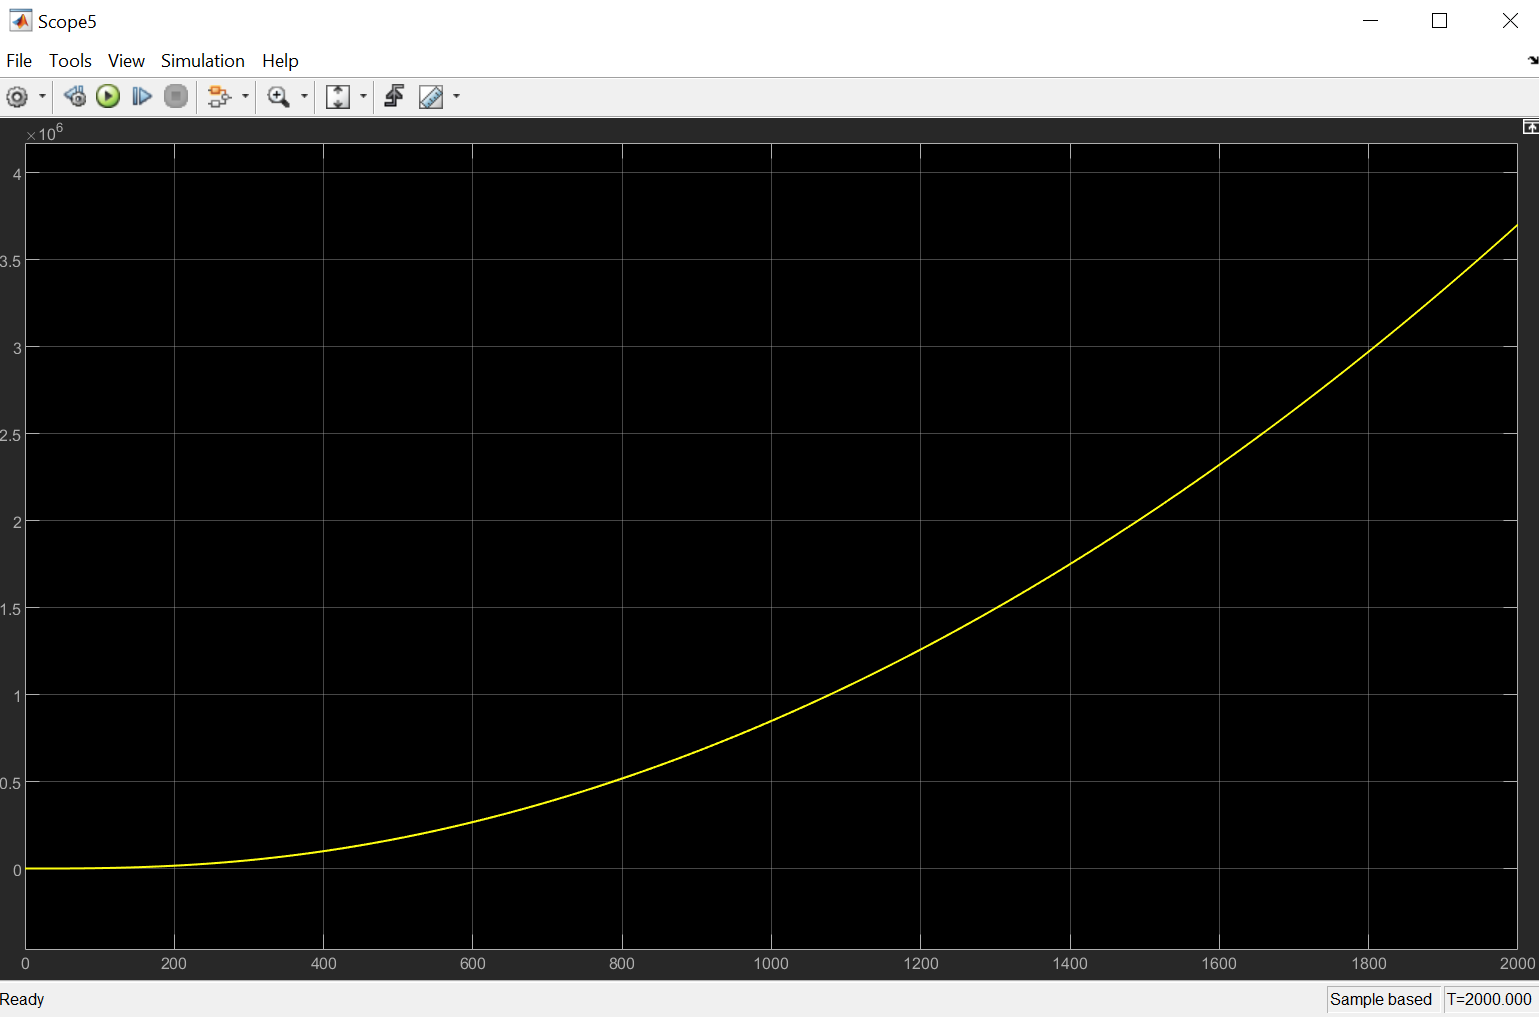
\includegraphics[scale=0.35]{images/parabolicResponse_PID_Simulink.png}
		\caption{Plot of Parabolic Response in Simulink After PID}
	\end{figure}
\end{frame}


\begin{frame}{MATLAB Results}
\begin{figure}[h!]
	\centering
	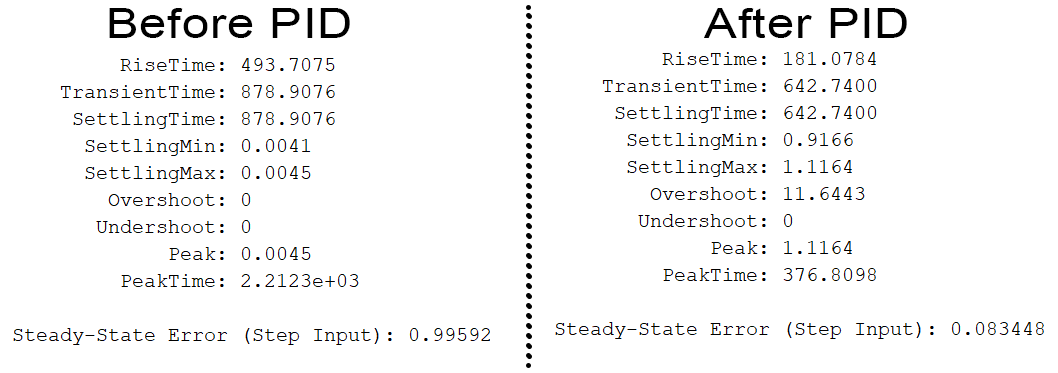
\includegraphics[scale=0.6]{images/SSE_MATLAB.png}
	\caption{Comparison of Step Response before and after PID Controller}
\end{figure}

\end{frame}


\begin{frame}{MATLAB Results}
\begin{figure}[h!]
	\centering
	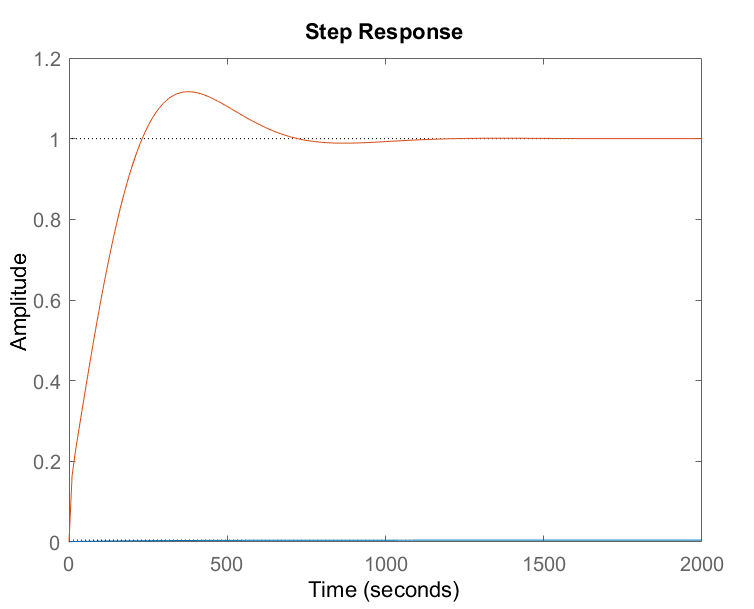
\includegraphics[scale=0.6]{images/stepResponse_PID_MATLAB.png}
	\caption{Plot of Step Response in MATLAB}
\end{figure}
\end{frame}

\begin{frame}{MATLAB Results}
\begin{figure}[h!]
	\centering
	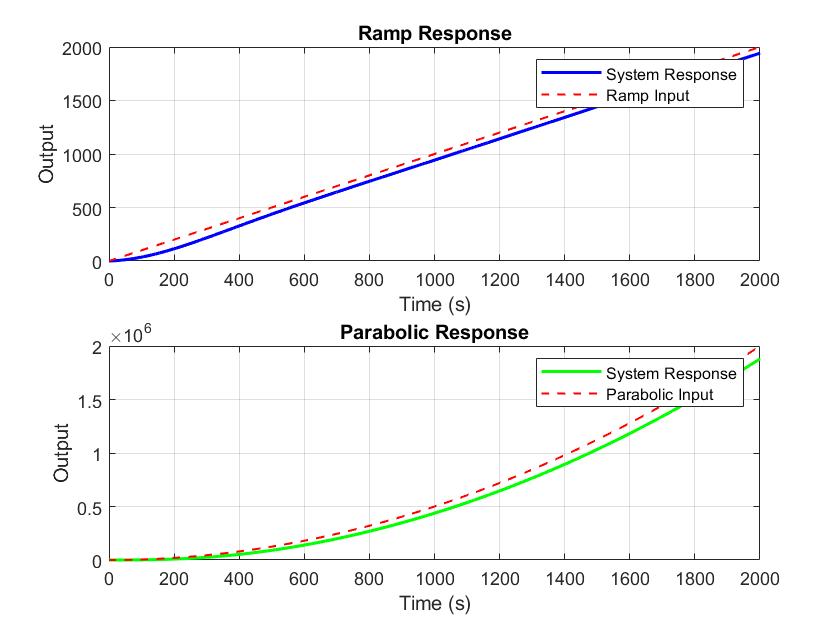
\includegraphics[scale=0.45]{images/rampparabolicResponse_PID_MATLAB.png}
	\caption{Plot of Step Response in MATLAB}
\end{figure}
\end{frame}



\end{document} 